% ============================================================================
%  Guia del Simulink del Segway. Version corta del modelo completo, enfocada
%  en entender el diagrama bloque por bloque.
%
%  Compilar DOS veces desde esta carpeta:
%     pdflatex -interaction=nonstopmode guia_simulink.tex
%
%  Las figuras las genera simulacion/segway_completo/exportar_diagramas.m
% ============================================================================
\documentclass[11pt,a4paper]{article}
\usepackage[utf8]{inputenc}
\usepackage[T1]{fontenc}
\usepackage[spanish,es-noshorthands]{babel}
\usepackage[margin=2cm]{geometry}
\usepackage{amsmath,amssymb}
\usepackage{graphicx}
\usepackage{booktabs}
\usepackage{xcolor}
\usepackage{tcolorbox}
\usepackage{enumitem}
\usepackage{caption}
\usepackage{titlesec}
\usepackage[colorlinks=true,linkcolor=blue!50!black,urlcolor=blue!50!black]{hyperref}

\graphicspath{{../../simulacion/segway_completo/diagramas/}%
              {../../simulacion/segway_completo/resultados/}}

\setlength{\parskip}{5pt}
\setlength{\parindent}{0pt}
\captionsetup{font=small,labelfont=bf}
\titlespacing*{\section}{0pt}{14pt}{6pt}

\definecolor{azulp}{RGB}{31,95,168}
\definecolor{verdep}{RGB}{27,94,32}
\definecolor{rojop}{RGB}{198,40,40}

\newtcolorbox{idea}{colback=azulp!6,colframe=azulp,boxrule=0.9pt,
  left=7pt,right=7pt,top=5pt,bottom=5pt,arc=2pt,
  fonttitle=\bfseries,title=En una frase}
\newtcolorbox{ojo}{colback=rojop!5,colframe=rojop,boxrule=0.9pt,
  left=7pt,right=7pt,top=5pt,bottom=5pt,arc=2pt,
  fonttitle=\bfseries,title=Ojo}
\newtcolorbox{probar}{colback=verdep!5,colframe=verdep,boxrule=0.9pt,
  left=7pt,right=7pt,top=5pt,bottom=5pt,arc=2pt,
  fonttitle=\bfseries,title=Para probar}

\newcommand{\bloque}[1]{\textsf{\textbf{#1}}}

\title{\vspace{-1.8cm}\huge Guía del Simulink del Segway\\[8pt]
\large Qué es cada bloque, qué significa cada señal y qué tocar para probar\\[12pt]
\normalsize Versión corta de \texttt{modelo\_del\_segway.pdf}, enfocada sólo en el diagrama}
\author{Grupo 4 --- Robótica II, UNCUYO}
\date{21 de octubre de 2026}

\begin{document}
\maketitle
\thispagestyle{empty}

\begin{idea}
El modelo son \textbf{seis bloques en fila}. Se lee de izquierda a derecha y lo que vuelve
del último al segundo cierra el lazo. Abrís un solo archivo y apretás Run.
\end{idea}

\vspace{-4pt}
\section*{En un minuto}

\begin{center}
\begin{tabular}{@{}ll@{}}
\toprule
\textbf{Qué abrir} & \texttt{simulacion/segway\_completo/INICIAR\_SEGWAY.m} \\
\textbf{Qué hacer} & apretar \textbf{Run}. Construye el modelo si falta, simula y verifica \\
\textbf{Qué tocar} & la \textbf{sección 2} de ese archivo: todo lo editable está junto ahí \\
\textbf{Dónde quedan las variables} & en el \textbf{workspace base}, que es de donde Simulink las lee \\
\bottomrule
\end{tabular}
\end{center}

\vspace{-6pt}
\section*{El diccionario: qué es cada símbolo}

Esto es lo primero que conviene tener claro, porque el diagrama usa estos nombres en todos lados.

\begin{center}
\small
\begin{tabular}{@{}llp{9.3cm}@{}}
\toprule
\textbf{Símbolo} & \textbf{Unidad} & \textbf{Qué es} \\
\midrule
$\tau$ (tau) & N$\cdot$m & \textbf{El par}: lo que el motor le tuerce a la rueda. Positivo
\textbf{empuja hacia adelante}. Por reacción, la rueda le devuelve $-\tau$ al cuerpo, y ésa es
la \emph{única} forma que tiene el robot de inclinarse a propósito \\
$U$ & V & la tensión que el control le manda a cada motor \\
$x$ & m & cuánto avanzó el eje de las ruedas \\
$v$ & m/s & velocidad de avance \\
$\varphi$ (phi) & rad & \textbf{la inclinación}, medida desde la dirección del centro de masa.
Positiva \textbf{hacia adelante}: el robot se inclina adelante para ir adelante \\
$\omega$ (omega) & rad/s & qué tan rápido se está inclinando \\
$\theta$ (theta) & rad & la postura de las patas: $10^\circ$ plegada, $40^\circ$ estirada \\
$\delta_G$ & rad & lo que hay \emph{entre} el ángulo del chasis y $\varphi$. Cambia con la
postura: va de $-9{,}09^\circ$ plegada a $-1{,}78^\circ$ estirada \\
\midrule
$a$ & kg & \textbf{masa efectiva de avance}. Vale 1,31 kg aunque el robot pese 0,96: la diferencia
es sobre todo la inercia del rotor vista a través de la reductora 1:20 (0,30 kg) y un poco el
giro de las ruedas (0,05) \\
$h$ & kg$\cdot$m & \textbf{masa por brazo}, $m_{cuerpo}\cdot\ell$. Es el \emph{acople}: si valiera
cero, avanzar e inclinarse serían independientes y el robot no se podría equilibrar con las ruedas \\
$j$ & kg$\cdot$m$^2$ & \textbf{inercia del cuerpo} alrededor del eje de la rueda \\
$k$ & N$\cdot$m/rad & \textbf{el par de la gravedad} por radián de inclinación. Es positivo: cuanto
más inclinado está, más lo voltea. Por eso el robot es inestable \\
\bottomrule
\end{tabular}
\end{center}

El estado completo es $z = [\,x;\ v;\ \varphi;\ \omega\,]$. Ésa es la señal que viaja por casi
todo el diagrama.

\clearpage
\section{El mapa: las seis etapas}

\begin{center}
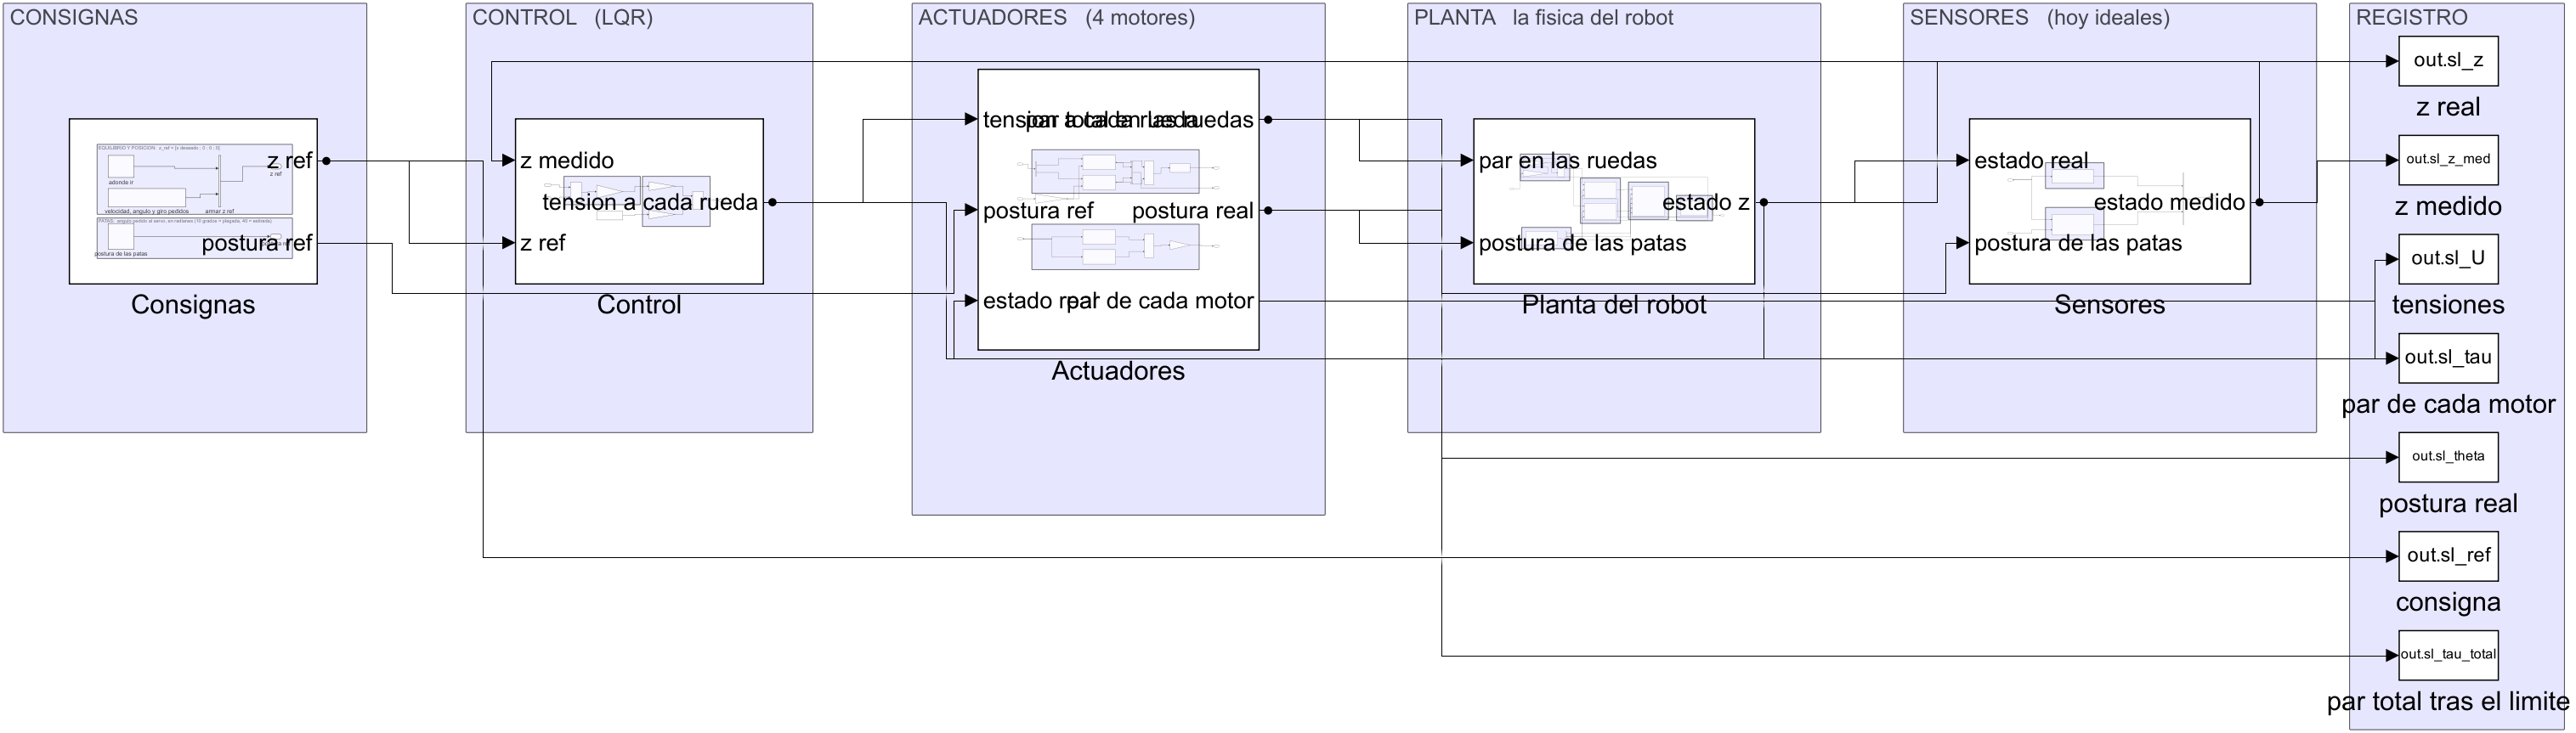
\includegraphics[width=\textwidth]{arriba.png}
\end{center}

\begin{center}
\small
\begin{tabular}{@{}lp{11.2cm}@{}}
\toprule
\bloque{Consignas} & adónde se le pide ir y en qué postura poner las patas \\
\bloque{Control} & un LQR: mira los cuatro estados a la vez y decide cuánta tensión mandarle a cada rueda \\
\bloque{Actuadores} & los cuatro motores, cada uno en su bloque \\
\bloque{Planta} & la física del robot \\
\bloque{Sensores} & lo que el robot puede medir. Hoy miden perfecto \\
\bloque{Registro} & saca las señales al workspace \\
\bottomrule
\end{tabular}
\end{center}

\begin{ojo}
Fijate que de la planta salen \textbf{dos} caminos.

El que va a \bloque{Sensores} y de ahí al control es \textbf{lo que el robot \emph{cree}} que le
pasa. El que va directo a \bloque{Actuadores} es \textbf{lo que de verdad} le pasa, porque el motor
siente la velocidad real de la rueda, no la medida.

Hoy los dos coinciden porque los sensores son ideales. Cuando les pongas ruido o retardo van a
separarse, y ahí se ve si el control aguanta.
\end{ojo}

\section{Consignas}

\begin{center}
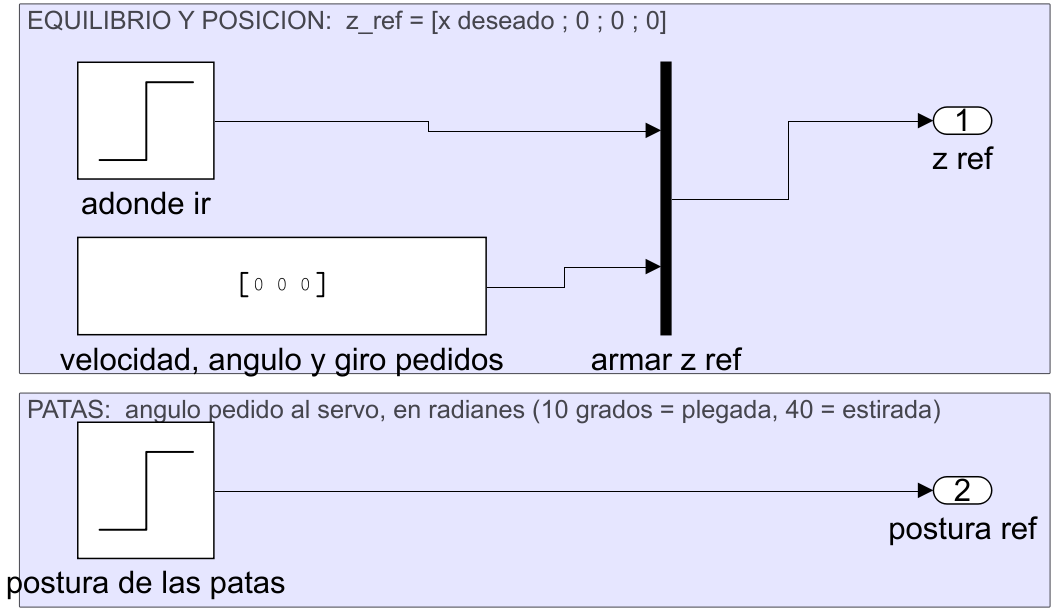
\includegraphics[width=\textwidth]{consignas.png}
\end{center}

Dos escalones, nada más. Uno dice adónde ir (se arma $z_{ref} = [x_{destino};\,0;\,0;\,0]$: se le
pide una posición y que lo demás quede en cero) y el otro en qué postura poner las patas.

Por defecto la postura es \textbf{constante}, así que el robot se comporta exactamente como el
modelo matemático verificado. Poniéndole un escalón, las patas se mueven.

\section{Control}

\begin{center}
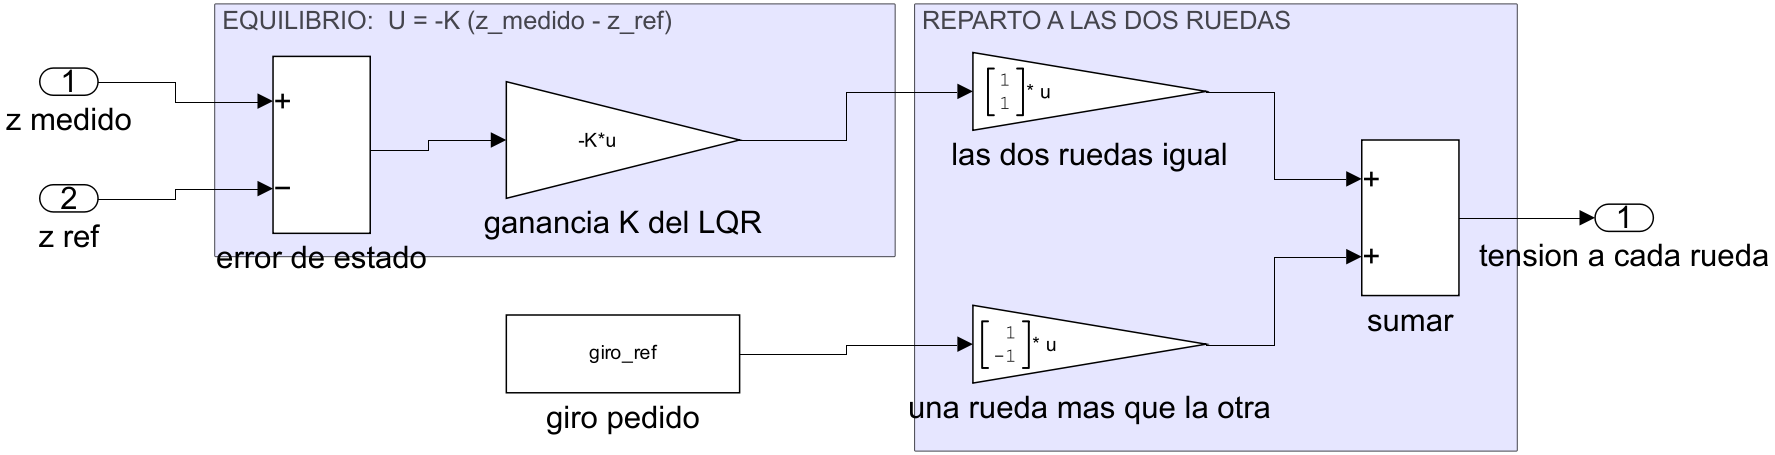
\includegraphics[width=\textwidth]{control.png}
\end{center}

\begin{idea}
$U = -K\,(z_{medido} - z_{ref})$. Una sola multiplicación de un vector de cuatro ganancias por el
error de los cuatro estados.
\end{idea}

$K = [\,-55{,}5\ \ -53{,}1\ \ -90{,}2\ \ -11{,}4\,]$, en voltios por (m, m/s, rad, rad/s).
Como $U = -K\,(z - z_{ref})$, los cuatro signos negativos quieren decir que una inclinación
hacia adelante pide tensión positiva, o sea empujar hacia adelante para meterse debajo del
cuerpo. Y la ganancia de posición es negativa por el cero de fase no mínima: para ir hacia
adelante, primero hay que empujar hacia atrás.

\textbf{Por qué una sola ganancia y no cuatro PID:} el robot tiene \emph{dos} coordenadas que
importan ($x$ y $\varphi$) y \emph{un} solo actuador. Realimentando sólo el ángulo se equilibra
pero se va caminando. $K$ mira los cuatro estados a la vez y los pesa.

El bloque de la derecha reparte a las dos ruedas. Hoy les da lo mismo a las dos, pero la entrada
de \emph{giro} ya está puesta en cero para el día que se quiera doblar: ahí cada rueda va a
recibir la suya y no hay que tocar nada más.

\clearpage
\section{Actuadores: los cuatro motores}

\begin{center}
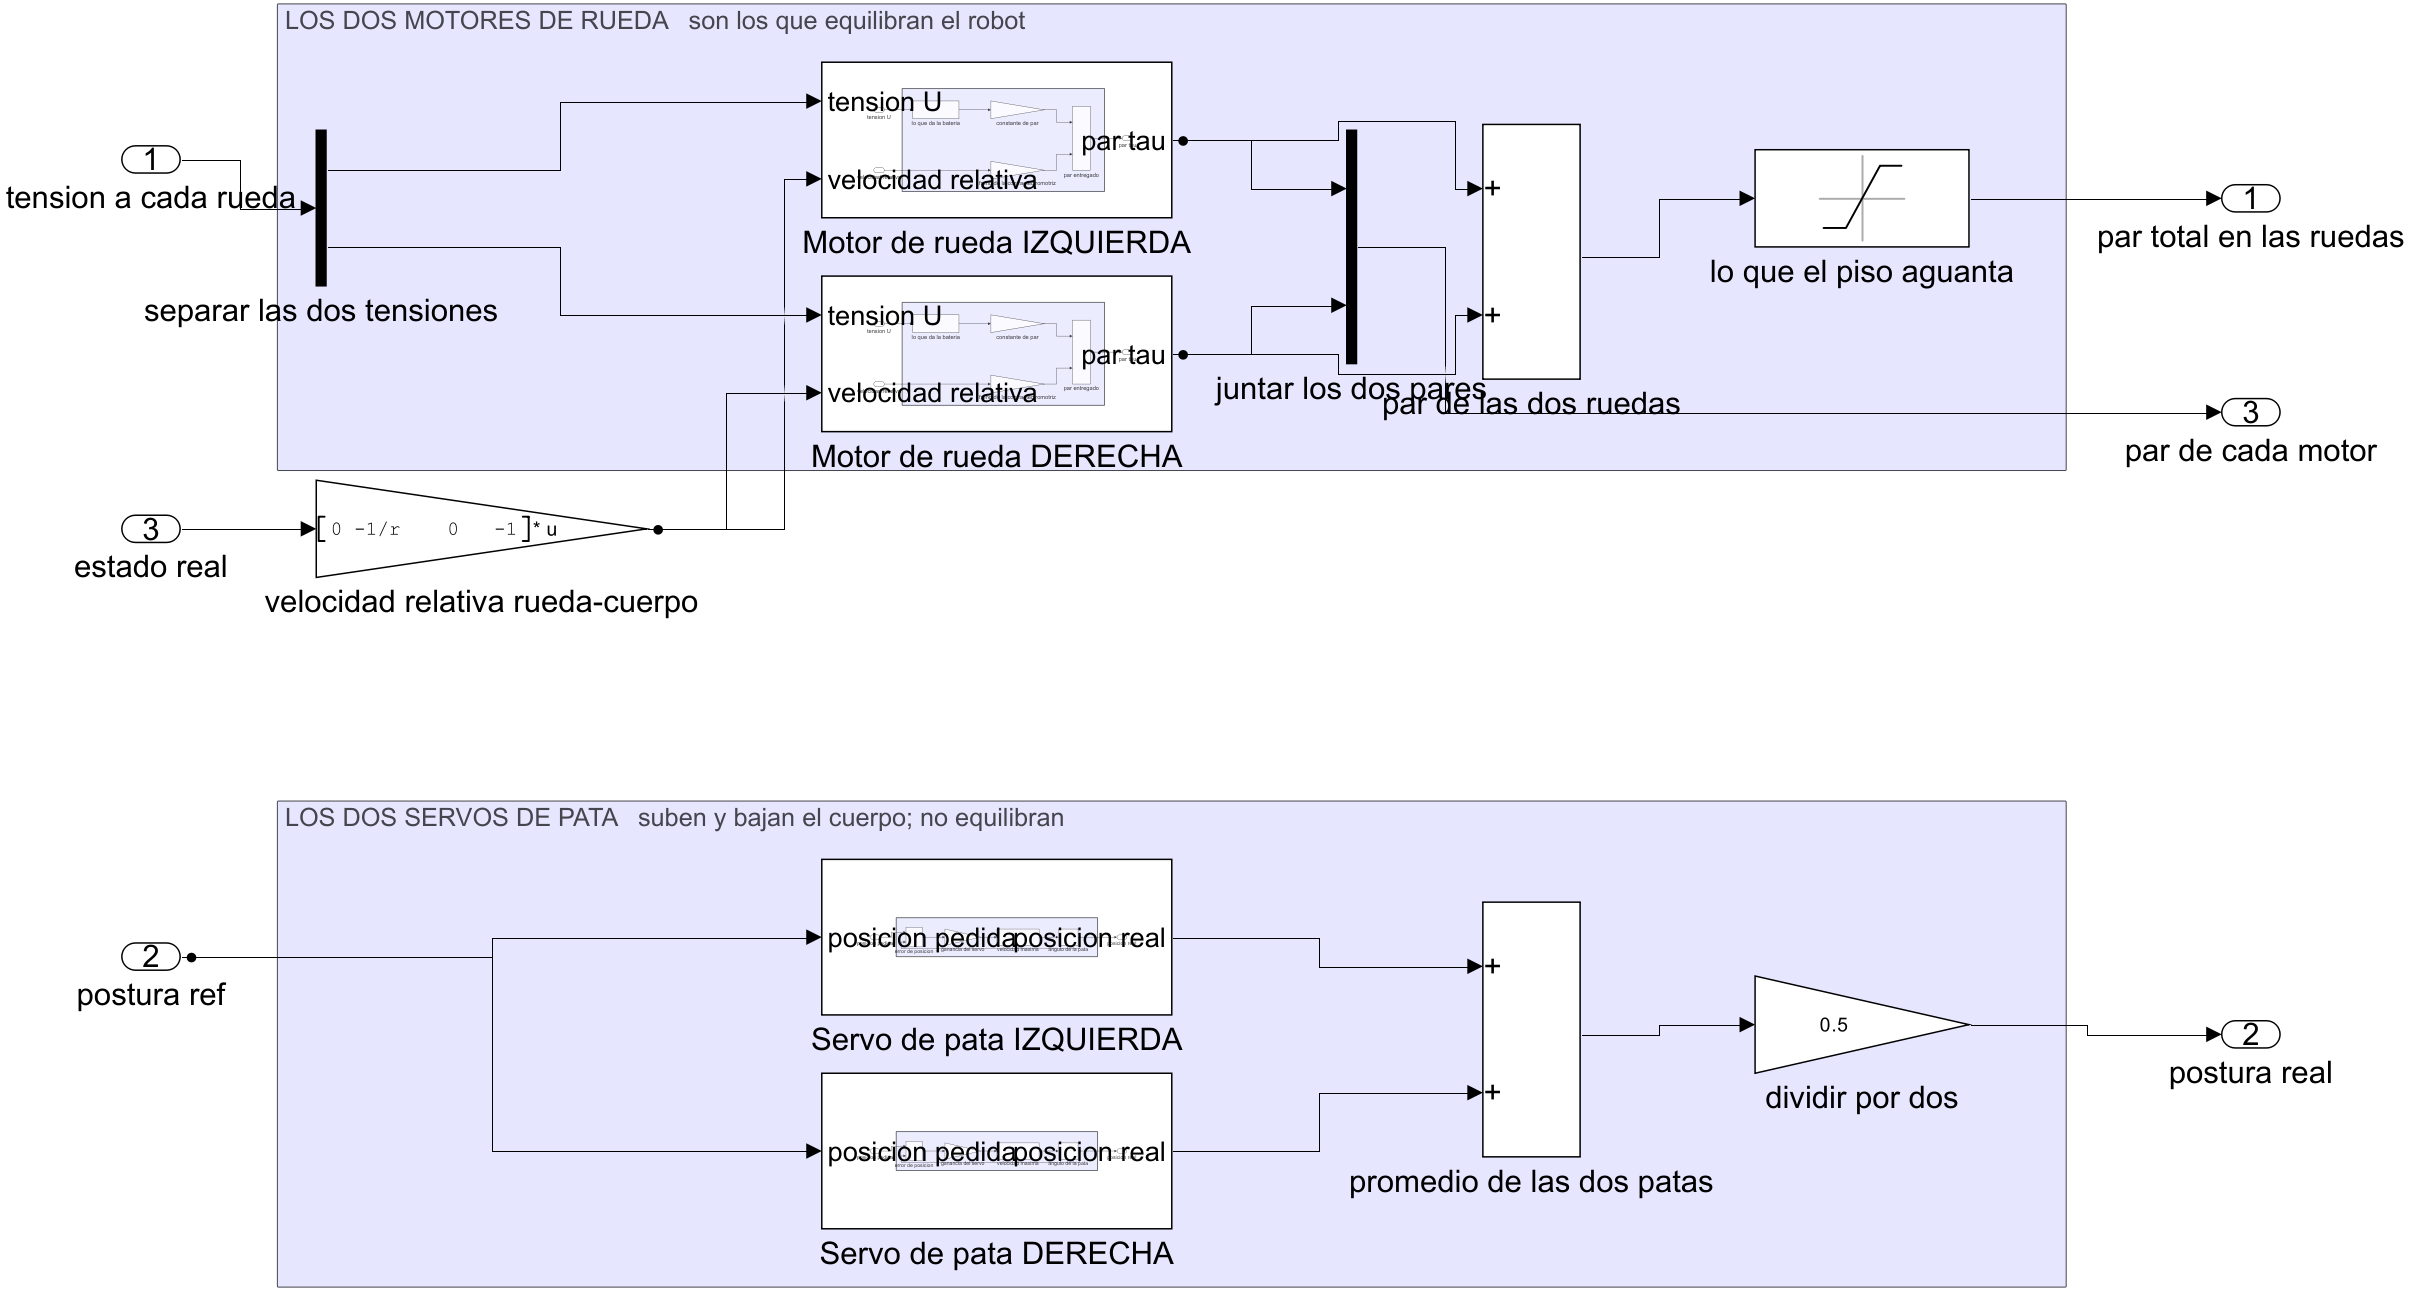
\includegraphics[width=\textwidth]{actuadores.png}
\end{center}

Arriba los dos motores de rueda, que son los que equilibran. Abajo los dos servos de pata, que
suben y bajan el cuerpo y \textbf{no} equilibran.

El bloque de la izquierda calcula la \emph{velocidad relativa rueda--cuerpo}, $-v/r - \omega$, que
es la que ven los motores. Después de sumar los dos pares viene la saturación del \emph{límite de
agarre}: por más par que haga el motor, el piso no transmite más de lo que la fricción aguanta.

\subsection*{Un motor de rueda}

\begin{center}
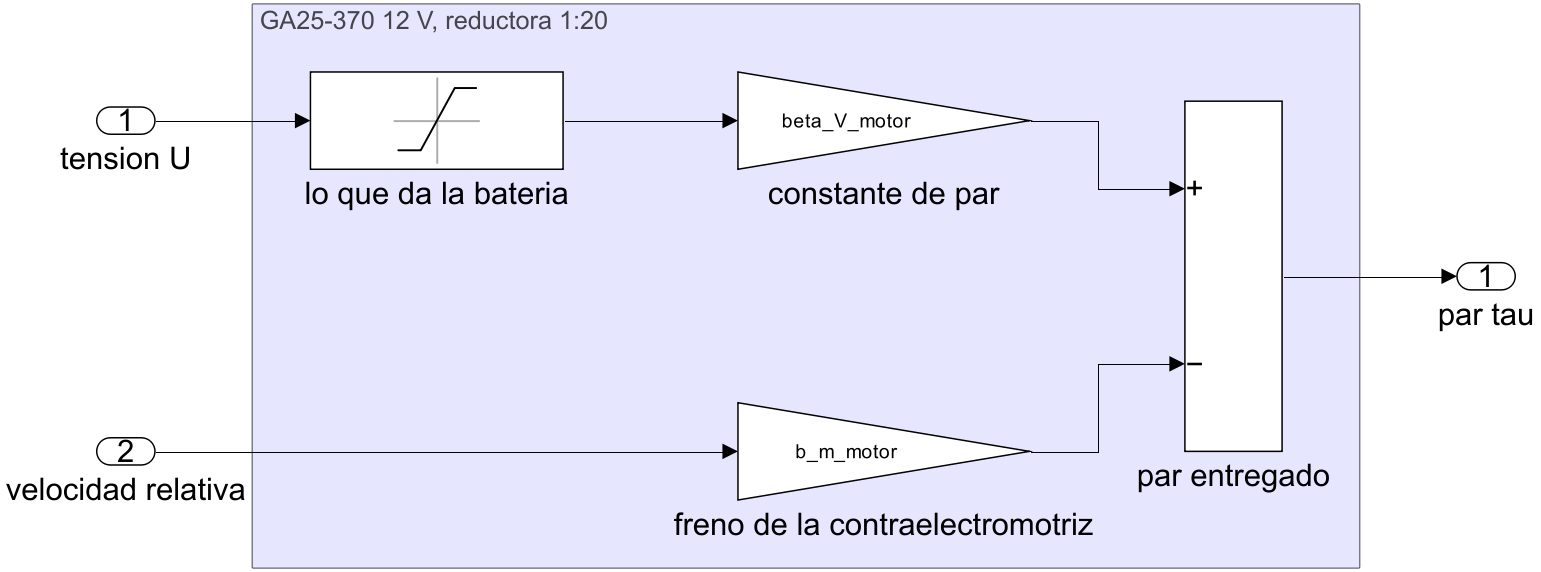
\includegraphics[width=\textwidth]{motor_rueda.png}
\end{center}

\[
\tau = \underbrace{\beta_V\,U}_{\text{lo que da}} \;-\; \underbrace{b_m\,\omega_{rel}}_{\text{lo que pierde}}
\]

El primer término es cuánto par da por cada voltio. El segundo es la \textbf{fuerza
contraelectromotriz}: cuanto más rápido gira la rueda respecto del cuerpo, menos par entrega. Sin
ese término el motor daría par infinito a cualquier velocidad; es el que le pone un techo de
1,23 m/s al robot.

La saturación de adelante es la batería: el control puede \emph{pedir} 16 V, pero entran 11,1.

\subsection*{Un servo de pata}

\begin{center}
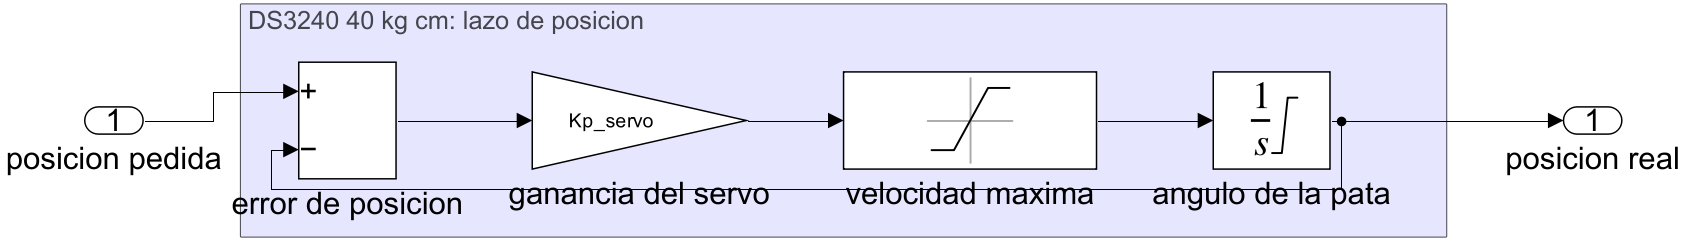
\includegraphics[width=\textwidth]{servo_pata.png}
\end{center}

Un servo ya trae su control adentro, así que no hay que diseñarle nada: sólo decirle a qué ángulo
ir. Lo que se ve es el lazo que el servo tiene de fábrica: compara la posición pedida con la que
tiene y se mueve a una velocidad proporcional al error, hasta su velocidad máxima.

Los topes del integrador son los topes \textbf{mecánicos} de la pata. Que estén ahí y no en una
saturación aparte evita que el ángulo se pase y después vuelva.

\clearpage
\section{Planta: la física}

\begin{center}
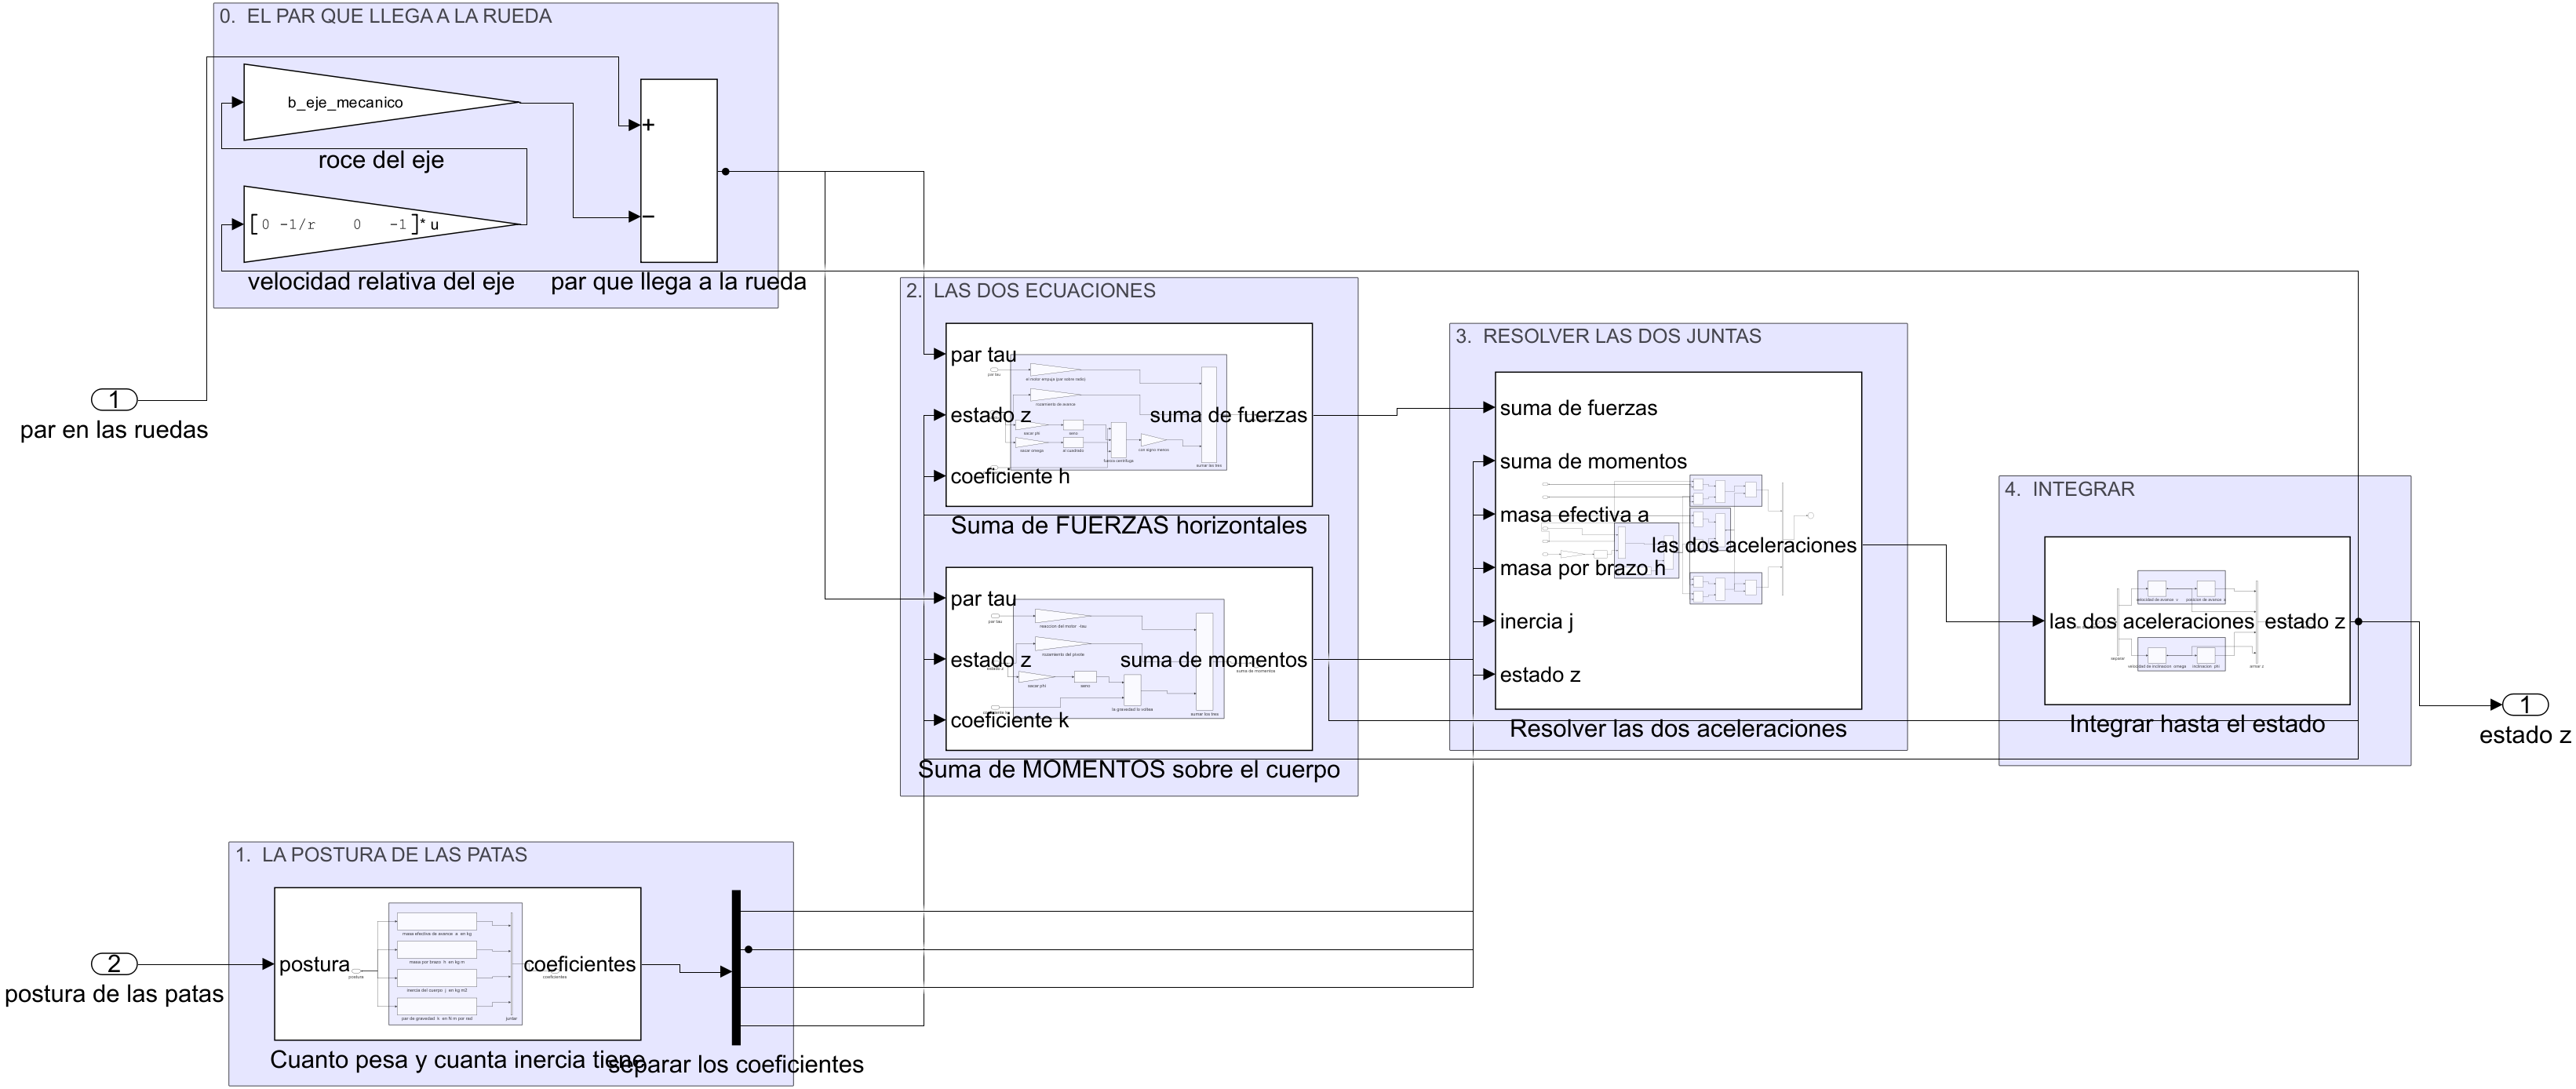
\includegraphics[width=\textwidth]{planta.png}
\end{center}

Cuatro etapas numeradas, en el orden en que se piensa el problema.

\begin{ojo}
\textbf{Por qué esto no es una cadena de integradores como en clase.}

En un cuerpo suelto: suma de fuerzas sobre masa da la aceleración, se integra dos veces y listo.
Acá no, porque el robot son \textbf{dos cuerpos pegados}: cuando la rueda acelera hacia adelante el
cuerpo se inclina hacia atrás, y cuando el cuerpo se inclina empuja la rueda.

Las dos aceleraciones aparecen en las \emph{dos} ecuaciones. Por eso primero se arma cada suma por
separado (etapa 2) y después se despejan las dos juntas (etapa 3).
\end{ojo}

\subsection*{Etapa 0 y 1: el par que llega, y los coeficientes}

Antes de todo se le descuenta al par el roce del eje, que es chiquito pero está.

\begin{center}
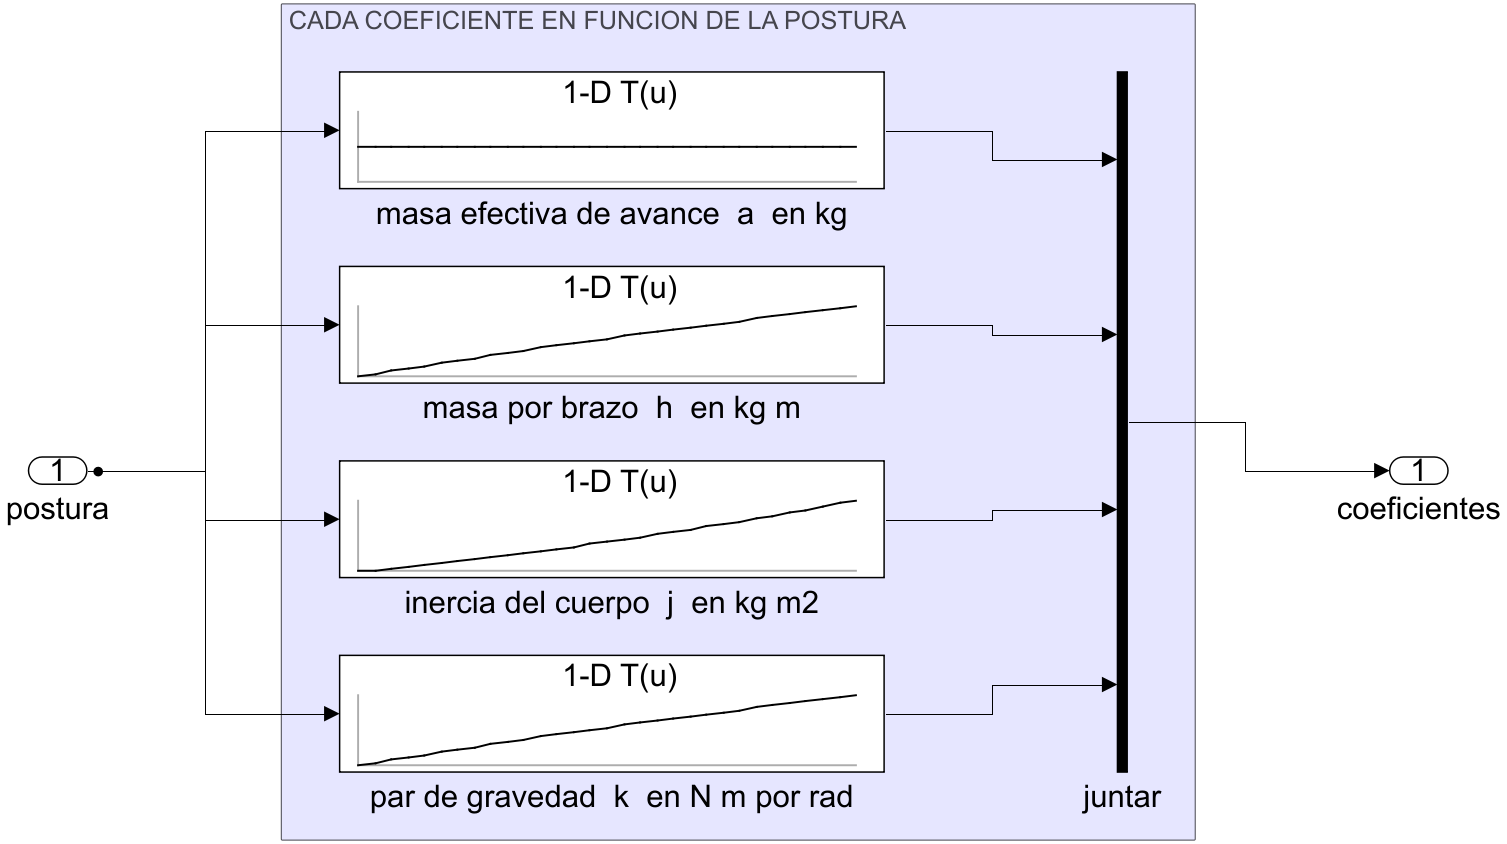
\includegraphics[width=\textwidth]{postura.png}
\end{center}

Después, la postura de las patas decide los cuatro coeficientes del cuerpo. Son tablas calculadas
al arrancar desde la fuente única de parámetros: al plegarse la pata el cuerpo baja, así que
cambian su brazo y su inercia. Con la postura constante devuelven siempre el mismo número.

\subsection*{Etapa 2: las dos ecuaciones}

\begin{center}
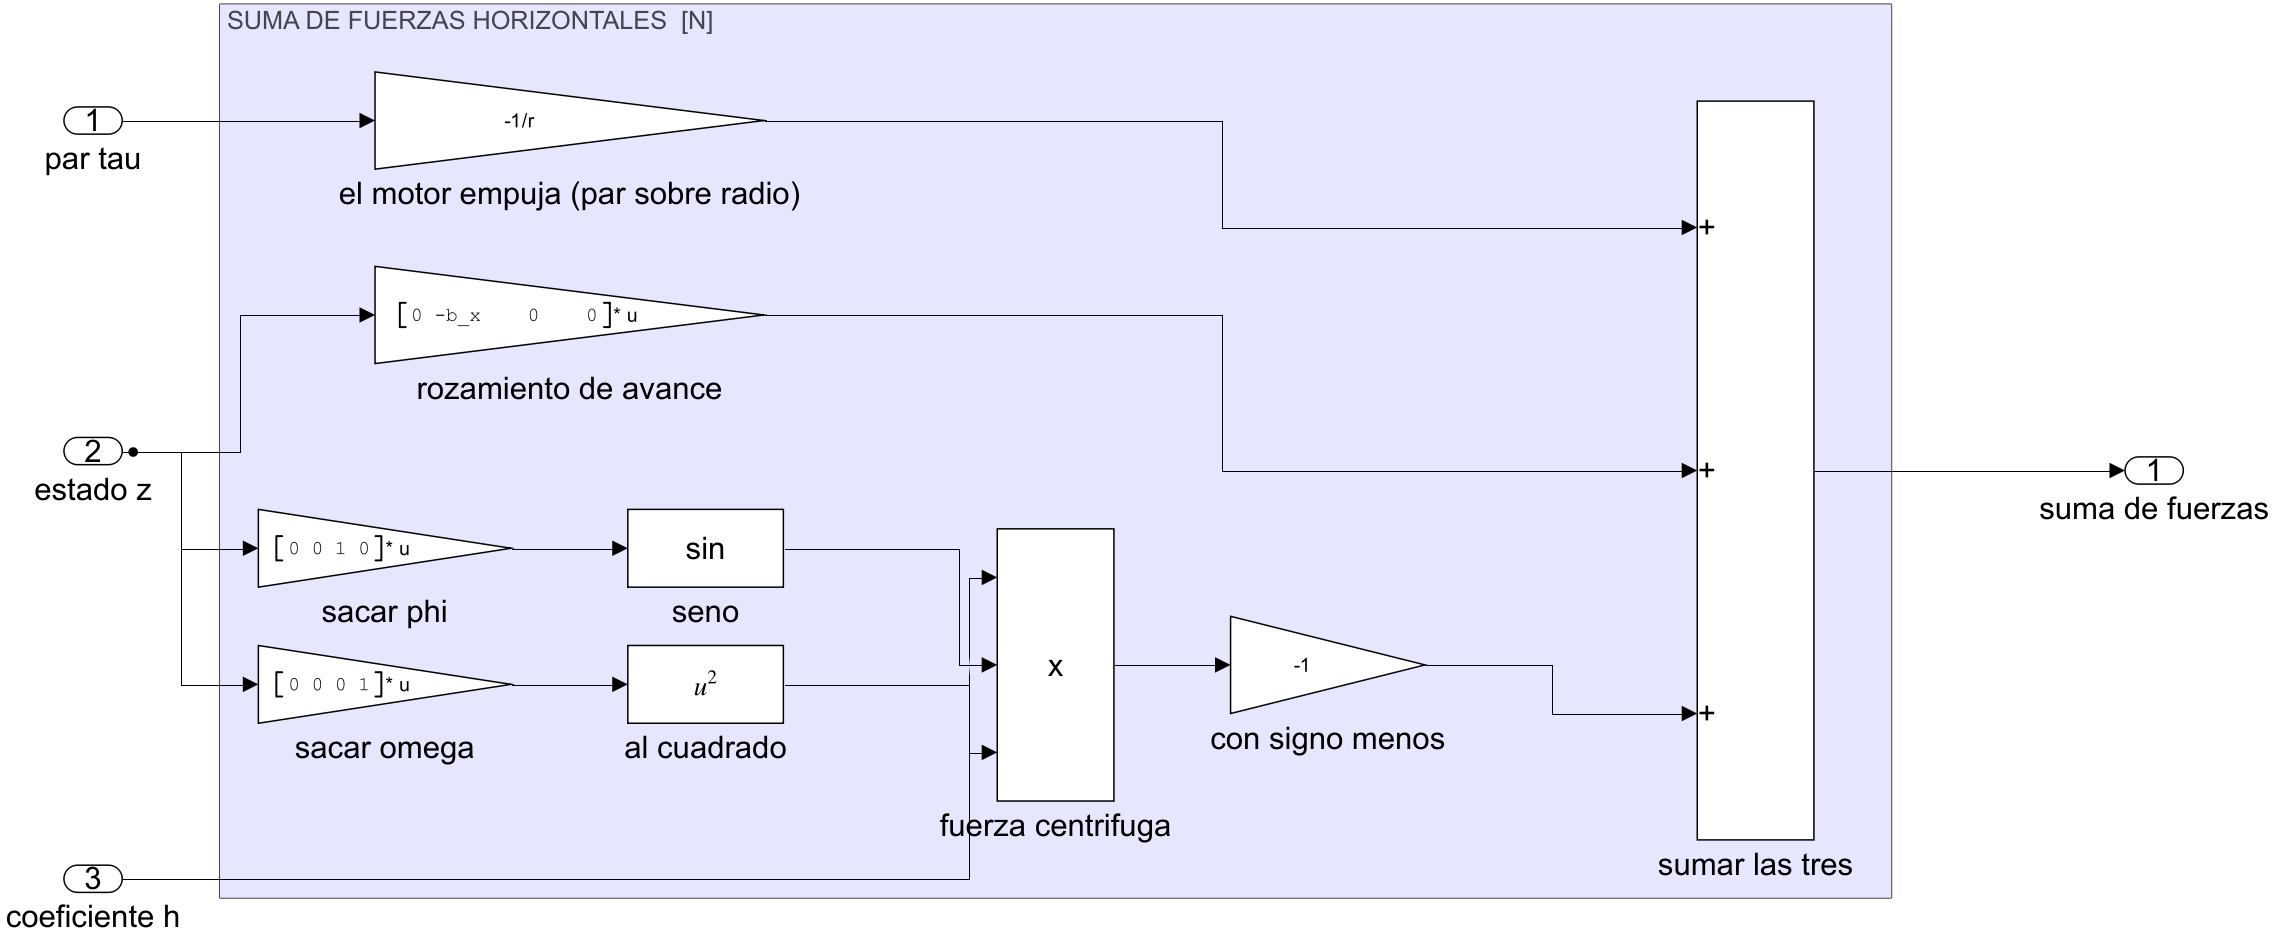
\includegraphics[width=\textwidth]{fuerzas.png}
\end{center}

\textbf{Suma de fuerzas horizontales}, en newtons. Tres términos:

\begin{center}
\small
\begin{tabular}{@{}lp{10.8cm}@{}}
\toprule
$+\tau/r$ & el par del motor, visto como fuerza en el contacto con el piso \\
$-b_x\,v$ & rozamiento de rodadura (hoy vale cero: no está medido) \\
$+h\sin\varphi\,\omega^2$ & la fuerza centrífuga del cuerpo girando inclinado. Es el \textbf{único
término no lineal} de todo el modelo, y sólo importa cuando el robot se inclina mucho y rápido \\
\bottomrule
\end{tabular}
\end{center}

\begin{center}
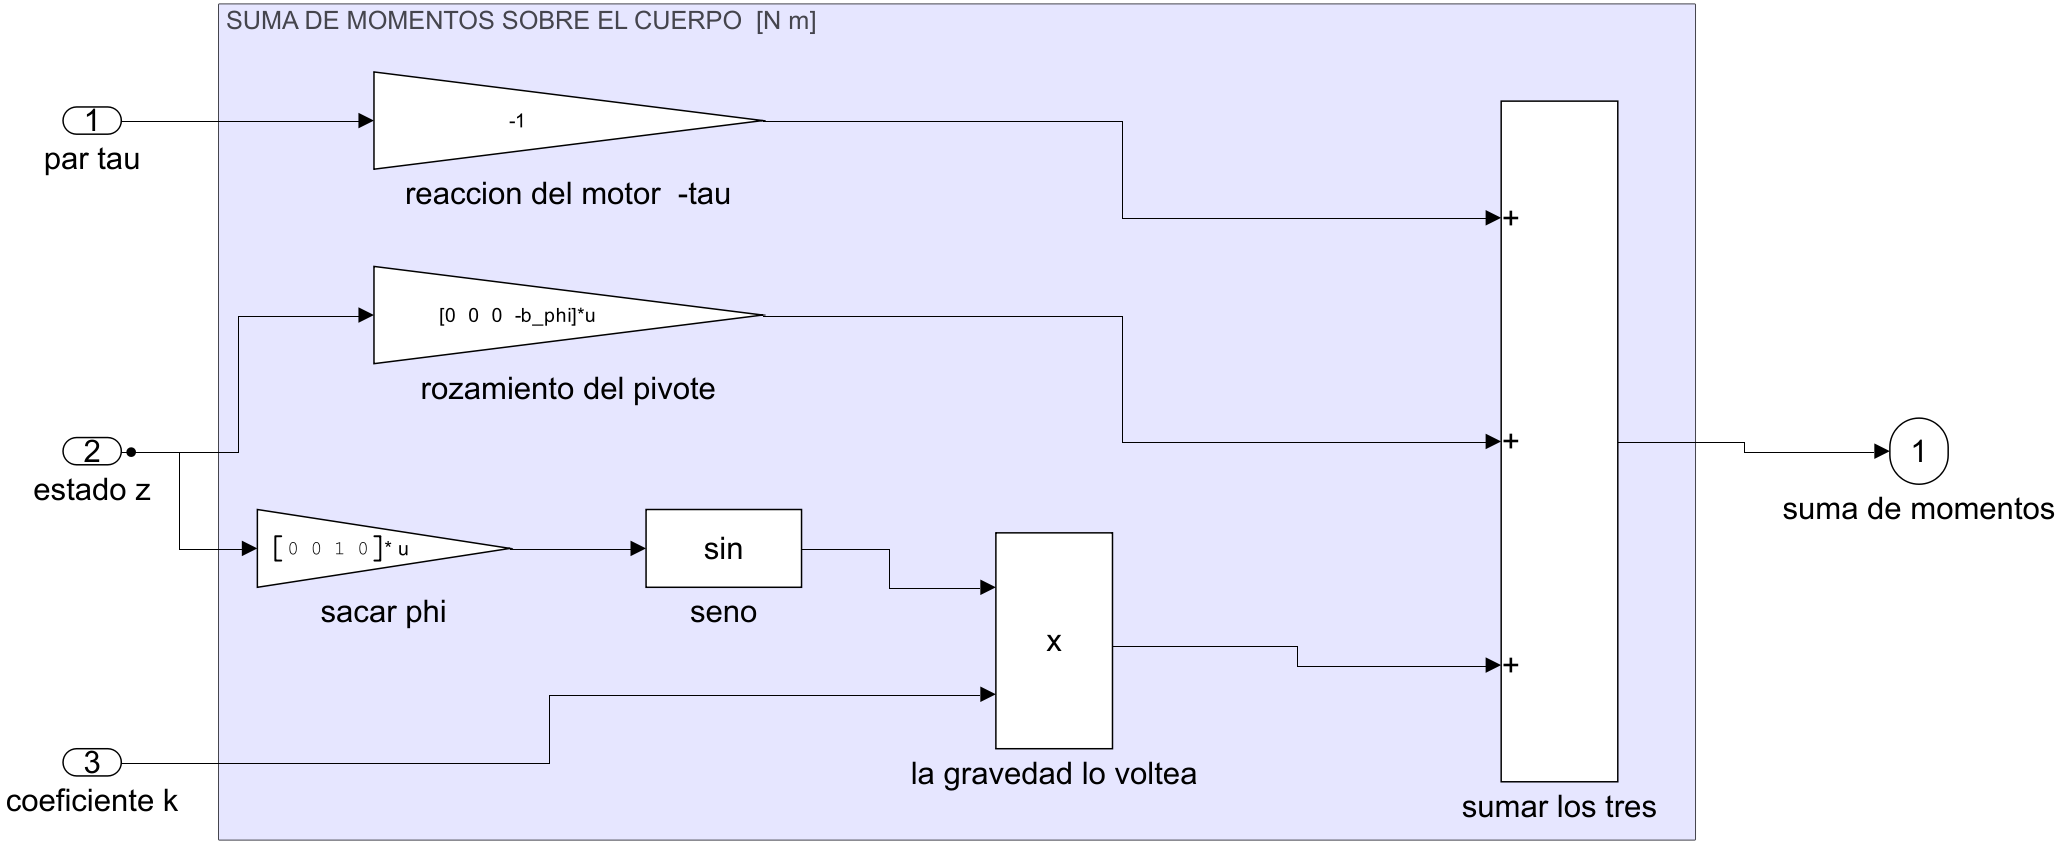
\includegraphics[width=\textwidth]{momentos.png}
\end{center}

\textbf{Suma de momentos sobre el cuerpo}, en N$\cdot$m. También tres:

\begin{center}
\small
\begin{tabular}{@{}lp{10.8cm}@{}}
\toprule
$-\tau$ & la \textbf{reacción} del motor. Si la rueda recibe $+\tau$, el cuerpo recibe $-\tau$.
Es la única manija que tiene el control para inclinar el robot \\
$-b_\varphi\,\omega$ & rozamiento del pivote (chiquito) \\
$+k\sin\varphi$ & la gravedad. El signo es \textbf{positivo}: cuanto más inclinado está, más lo
voltea. Ese signo es la razón de que el robot sea inestable \\
\bottomrule
\end{tabular}
\end{center}

\clearpage
\subsection*{Etapa 3: despejar las dos aceleraciones}

\begin{center}
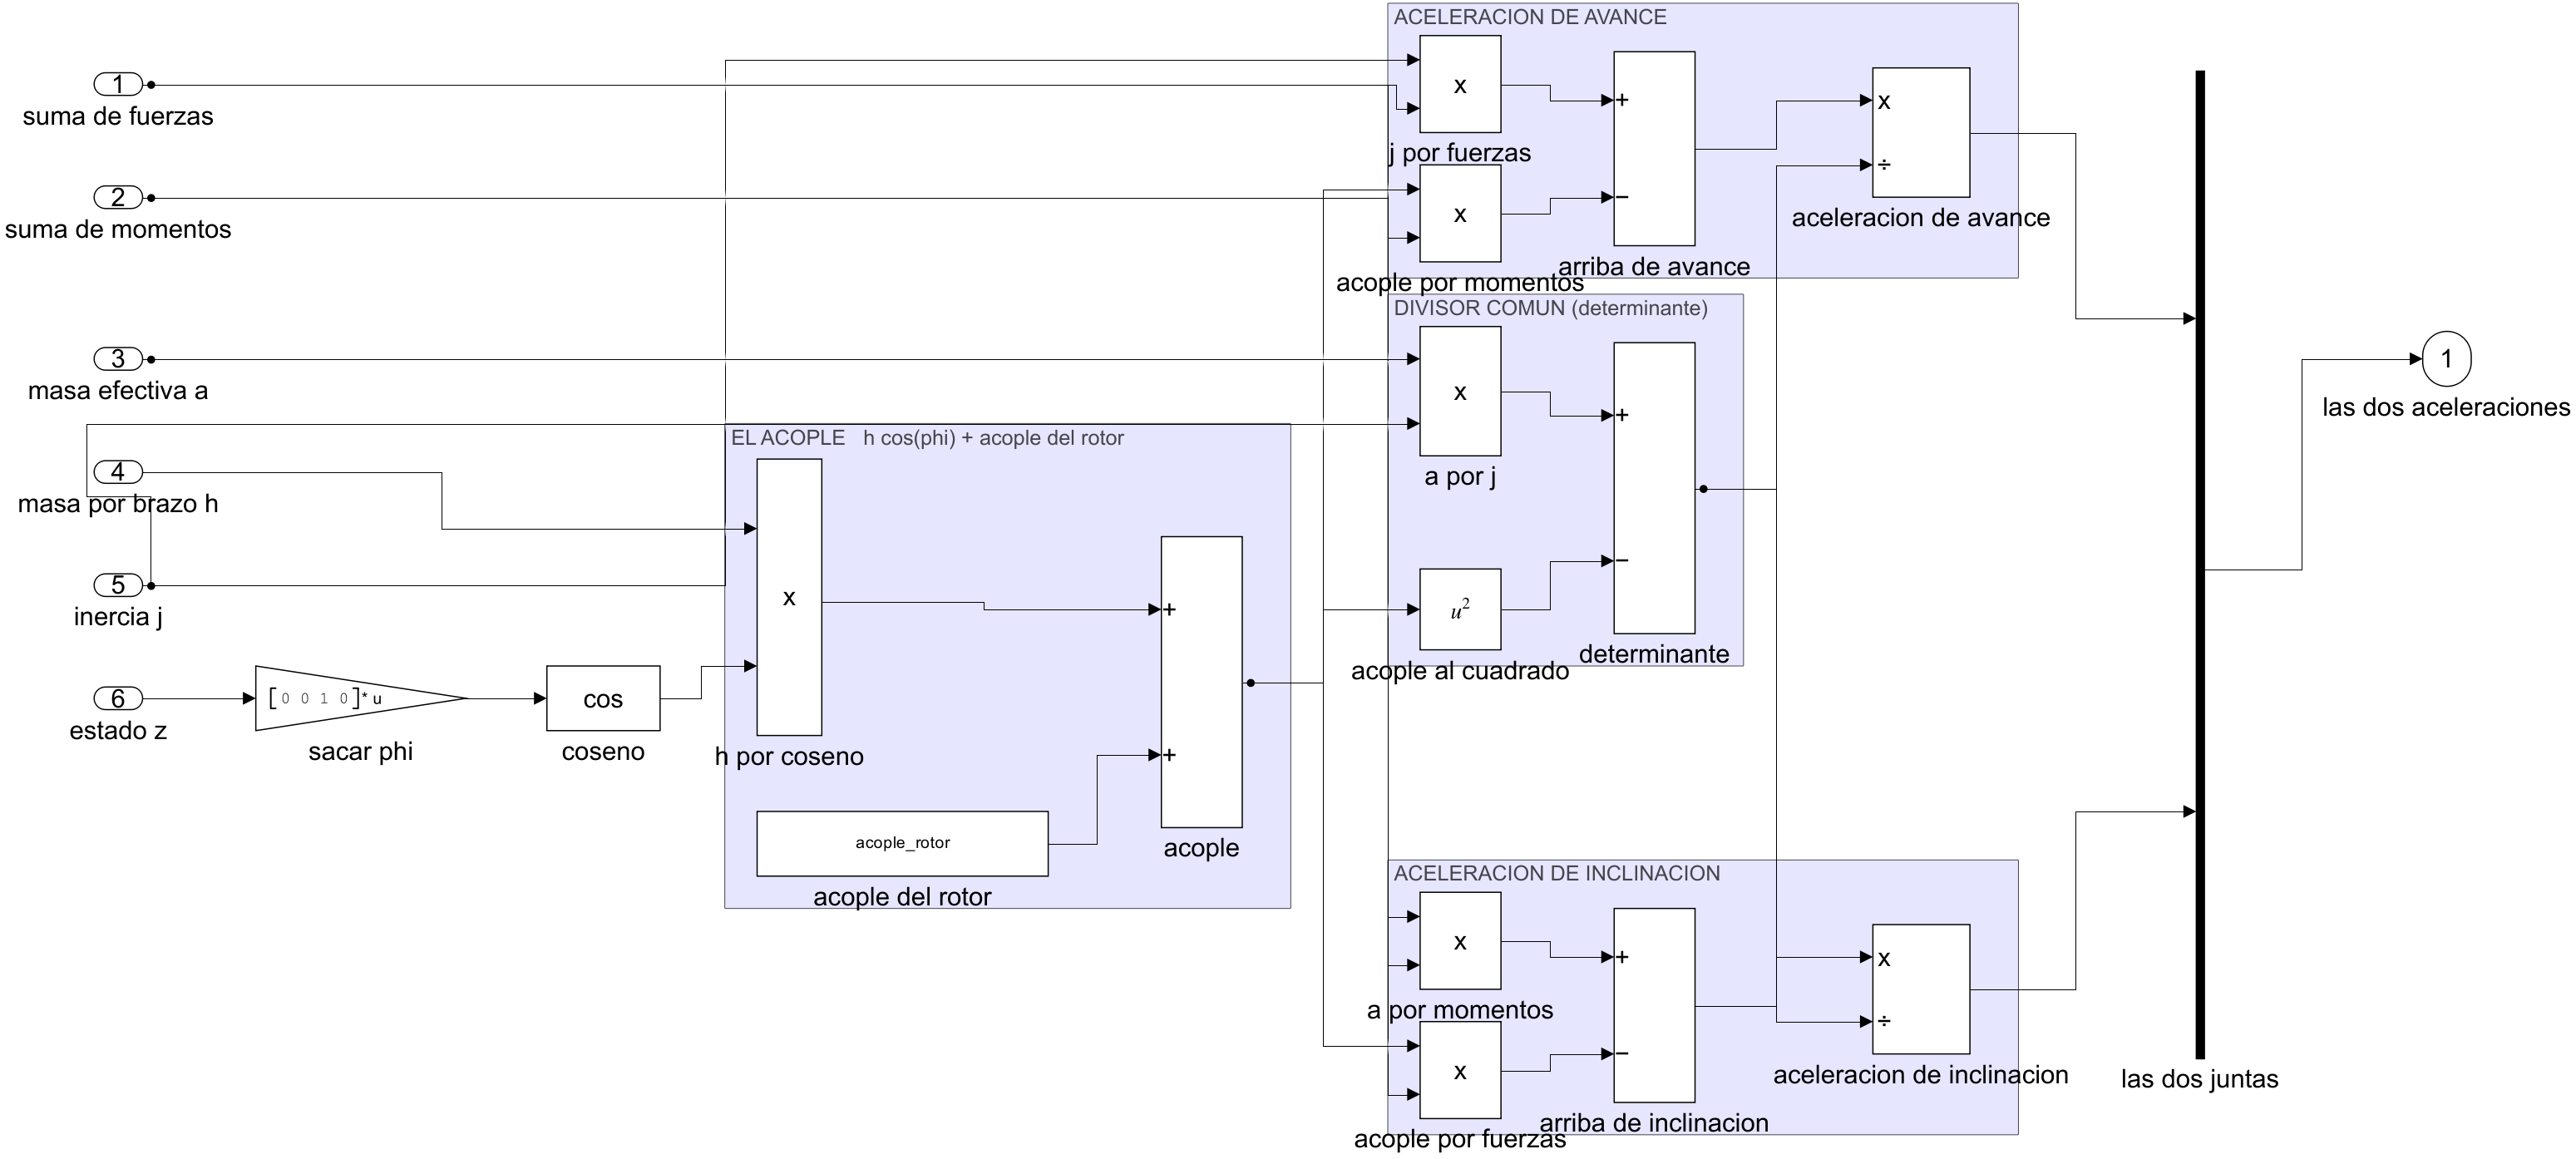
\includegraphics[width=\textwidth]{resolver.png}
\end{center}

Hay que despejar dos incógnitas de dos ecuaciones:

\[
\begin{bmatrix} a & \text{acople} \\ \text{acople} & j \end{bmatrix}
\begin{bmatrix} \ddot x \\ \ddot\varphi \end{bmatrix}
=
\begin{bmatrix} \text{suma de fuerzas} \\ \text{suma de momentos} \end{bmatrix}
\]

Con $2\times2$ se hace por \textbf{Cramer}, que es la regla de siempre: cada incógnita es un
determinante dividido por el determinante común.

\begin{align*}
\ddot x &= \frac{j\cdot\text{fuerzas} - \text{acople}\cdot\text{momentos}}{a\,j - \text{acople}^2} \\[4pt]
\ddot\varphi &= \frac{a\cdot\text{momentos} - \text{acople}\cdot\text{fuerzas}}{a\,j - \text{acople}^2}
\end{align*}

\textbf{El acople} vale $h\cos\varphi + \text{(una constante del rotor, que es negativa)}$, y es
el número que dice cuánto se afectan entre sí avanzar e inclinarse. Si fuera cero, las dos ecuaciones se separarían y
el robot no se podría equilibrar moviendo las ruedas, porque empujar la rueda no inclinaría el
cuerpo.

\subsection*{Etapa 4: integrar}

\begin{center}
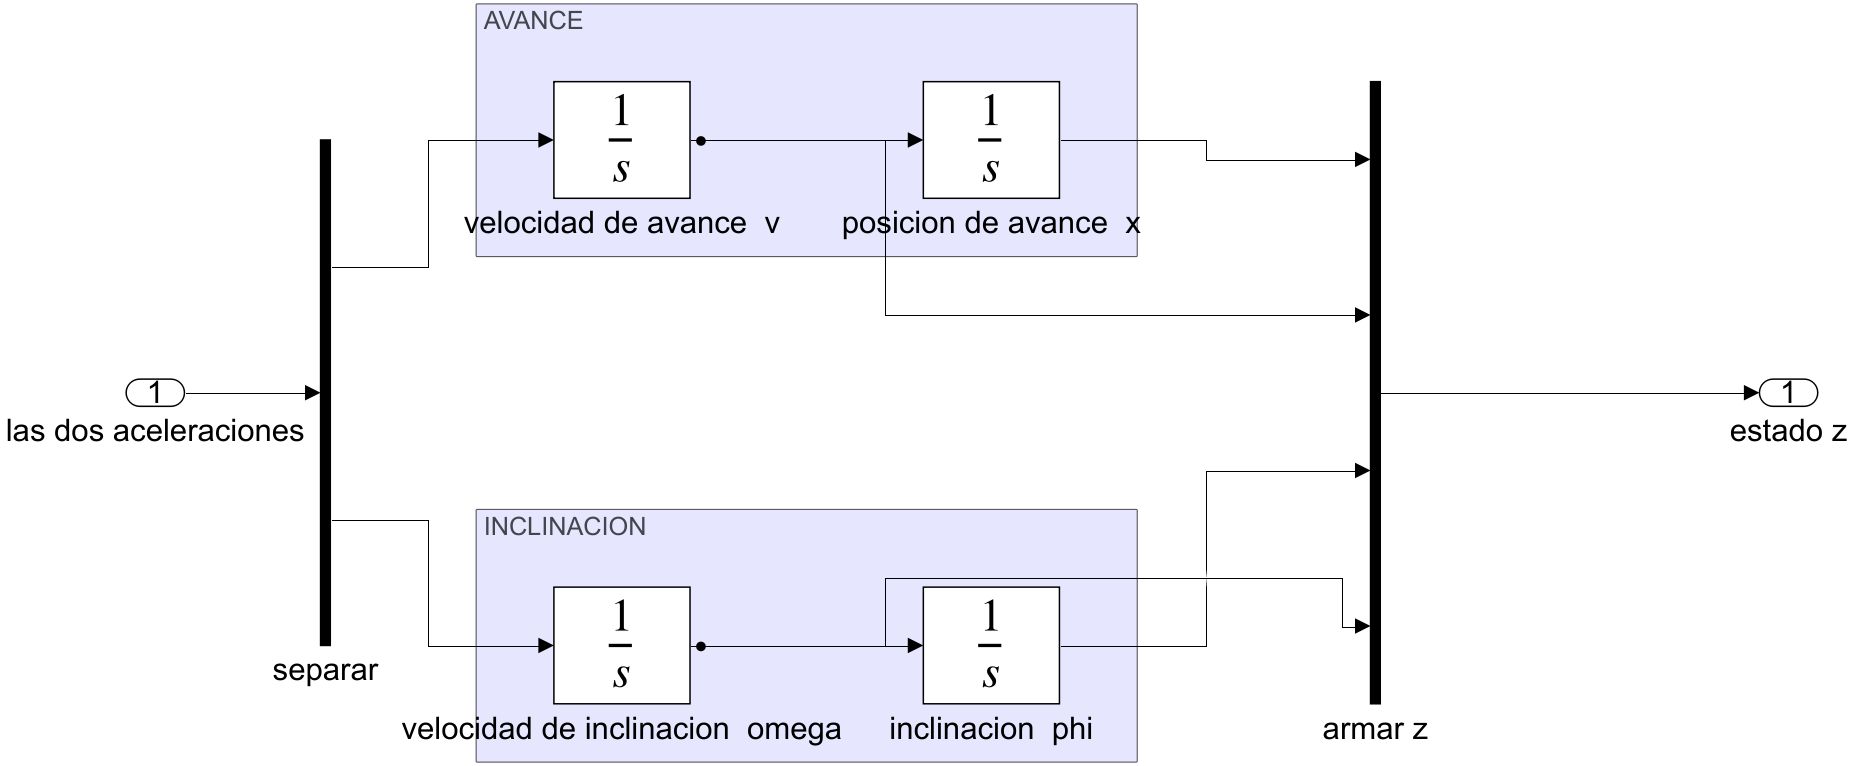
\includegraphics[width=\textwidth]{integrar.png}
\end{center}

Acá sí: dos cadenas de integradores, una para el avance y otra para la inclinación. Las
condiciones iniciales de los cuatro son el estado de arranque del robot.

\clearpage
\section{Sensores}

\begin{center}
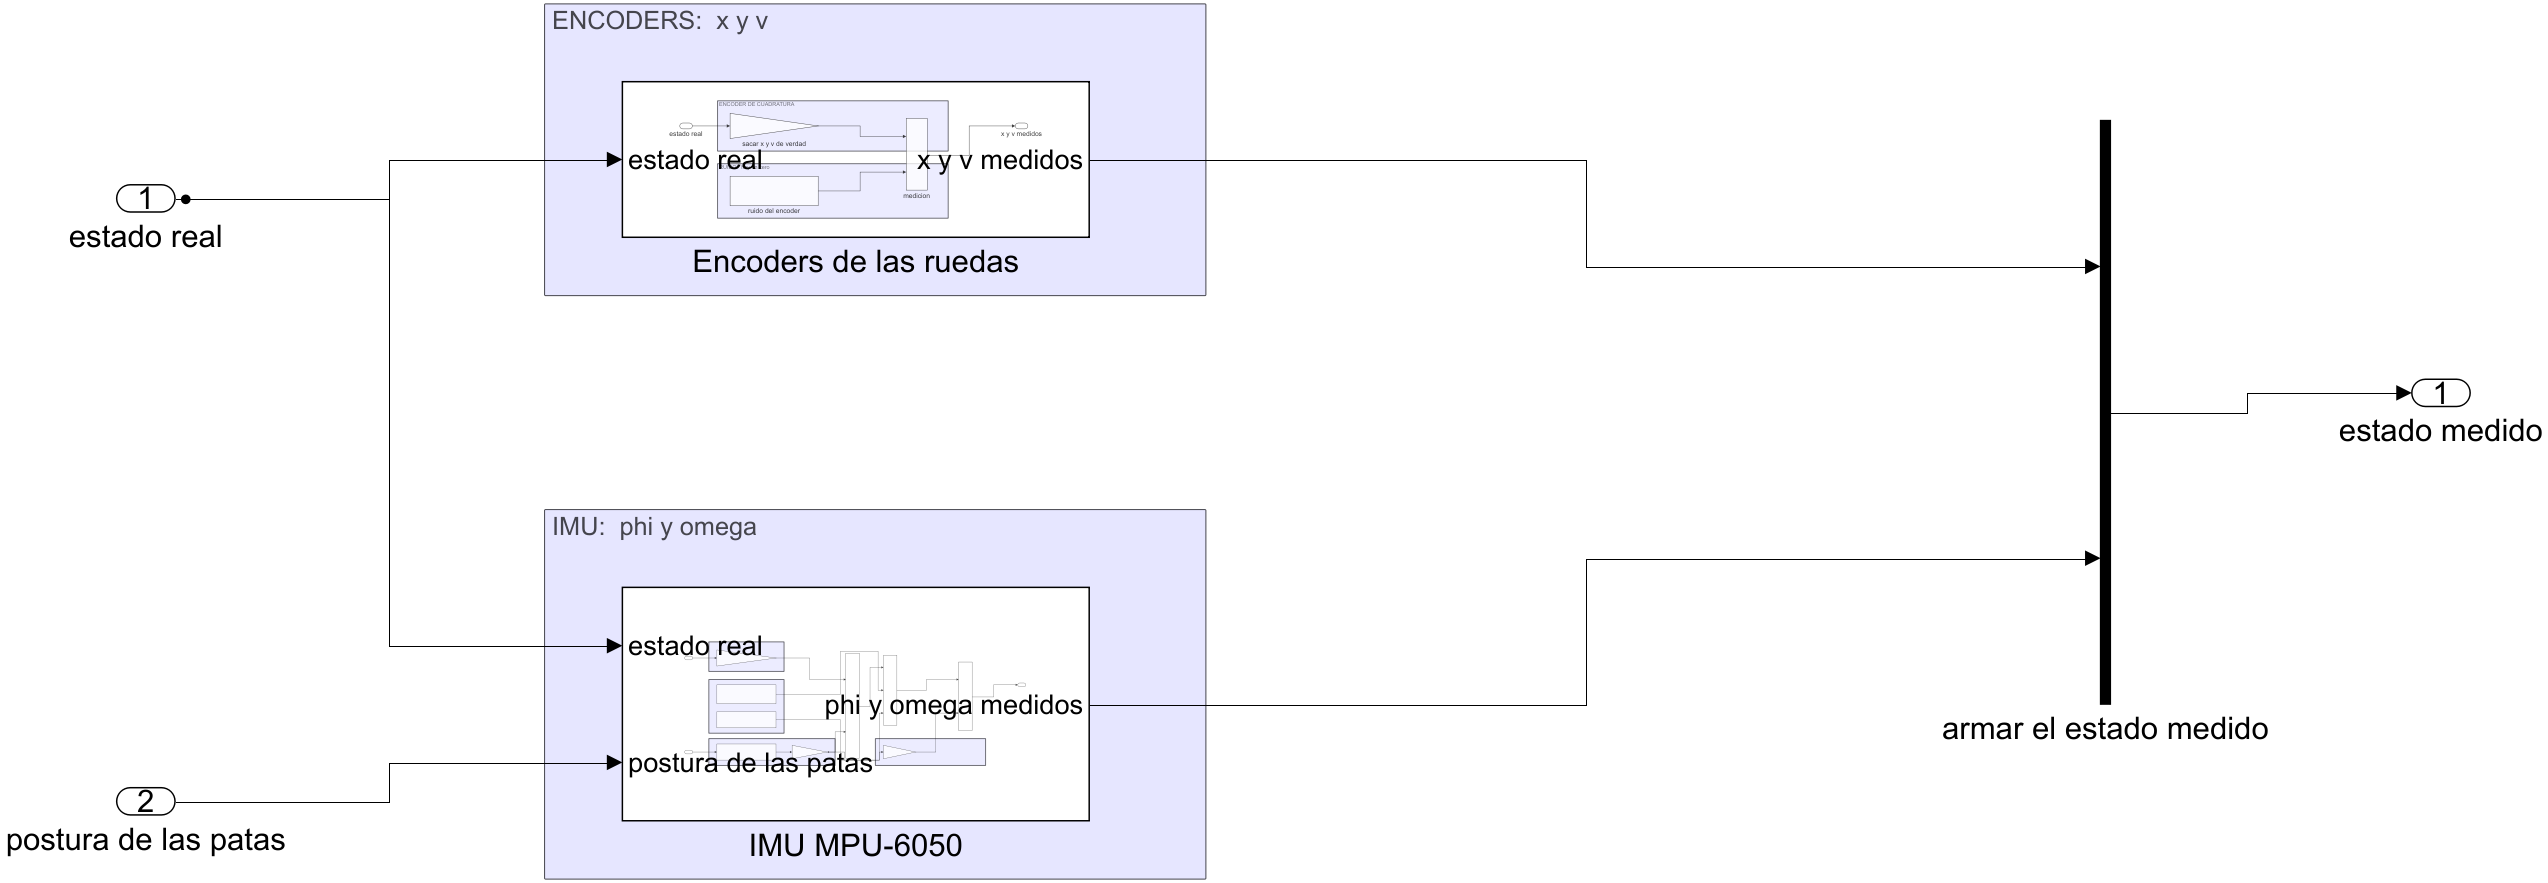
\includegraphics[width=\textwidth]{sensores.png}
\end{center}

Dos sensores: los encoders de las ruedas dan $x$ y $v$; la IMU da $\varphi$ y $\omega$. Hoy los dos
miden perfecto y el ruido está en cero, pero los lugares donde meter la realidad ya están puestos.

\subsection*{La IMU, y la trampa más fácil de todo el modelo}

\begin{center}
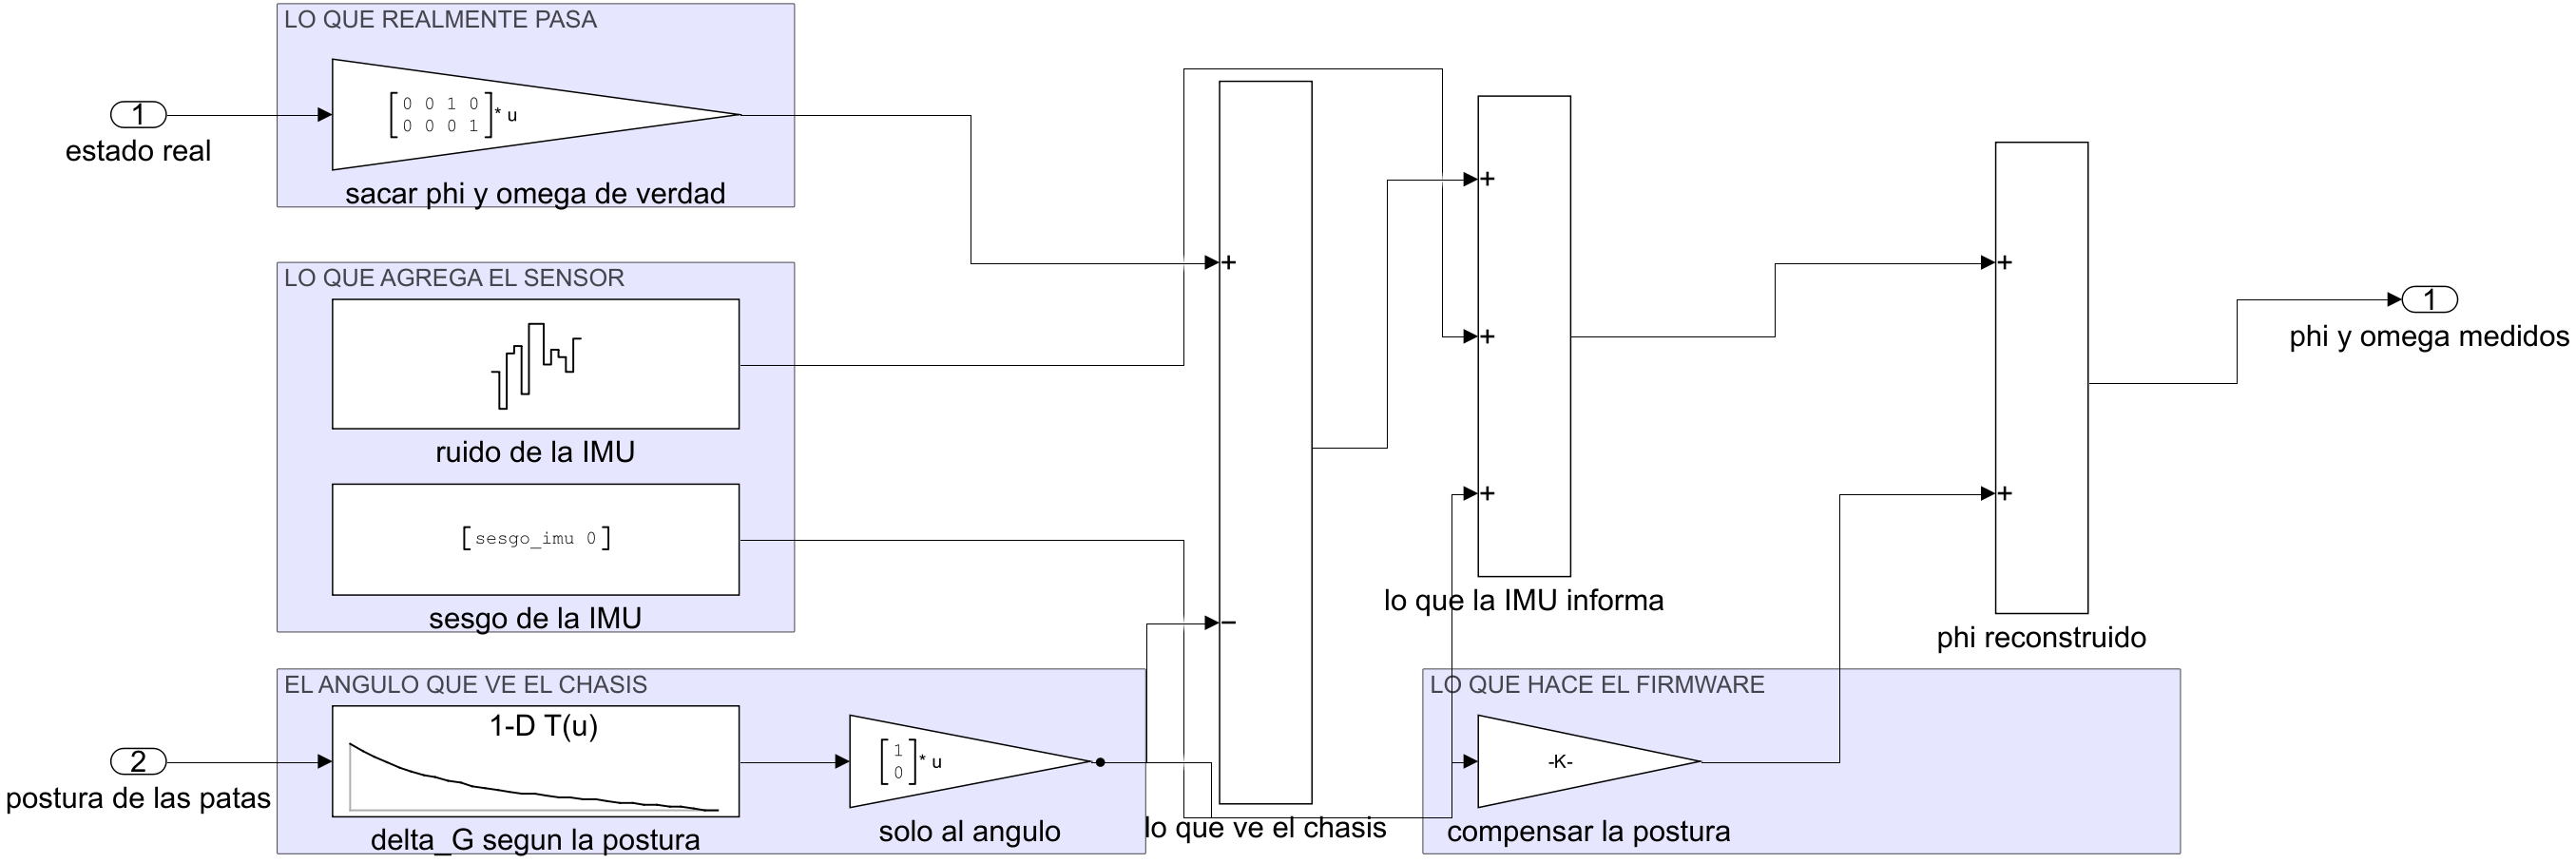
\includegraphics[width=\textwidth]{imu.png}
\end{center}

\begin{ojo}
\textbf{$\varphi$ NO es el ángulo del chasis.}

$\varphi$ se mide desde la dirección del centro de masa, y entre el chasis y esa dirección hay un
ángulo $\delta_G$. El problema es que $\delta_G$ \textbf{cambia con la postura de las patas}: vale
$-9{,}09^\circ$ con la pata plegada y $-1{,}78^\circ$ con la pata estirada.

O sea que al mover las patas, \textbf{el cero del ángulo se corre más de 7 grados}.
\end{ojo}

Por eso el bloque tiene tres partes: lo que realmente pasa, lo que le agrega el sensor (ruido y
sesgo), y lo que hace el firmware, que es volver a sumarle $\delta_G$ para recuperar $\varphi$.

Si el firmware no lo compensa, el control cree que el robot está inclinado cuando no lo está y sale
a corregir: el robot se va \textbf{21 cm} de donde estaba cada vez que cambia de postura.
Compensando, se queda en cero.

\section{Cómo correrlo}

Abrís \texttt{INICIAR\_SEGWAY.m} y apretás Run. Lo que conviene tocar está todo junto en la
\textbf{sección 2}:

\begin{center}
\small
\begin{tabular}{@{}llp{7.6cm}@{}}
\toprule
\textbf{Variable} & \textbf{Por defecto} & \textbf{Qué cambia} \\
\midrule
\texttt{postura\_deg} & 25 & en qué postura se diseña el control \\
\texttt{phi0\_deg} & 5 & de qué inclinación arranca \\
\texttt{x\_destino} & 0,30 m & adónde se le pide ir (0 = quedarse quieto) \\
\texttt{theta\_pata\_fin} & igual a la inicial & si las patas se mueven o no \\
\texttt{giro\_ref} & 0 & diferencia de tensión entre las dos ruedas \\
\texttt{ruido\_imu\_angulo} & 0 & ruido del ángulo de la IMU \\
\texttt{ruido\_encoder\_x} & 0 & ruido de posición del encoder \\
\texttt{sesgo\_imu} & 0 & error constante de la IMU, en radianes \\
\texttt{compensar\_delta\_G} & 1 & si el firmware corrige el ángulo según la postura \\
\bottomrule
\end{tabular}
\end{center}

Al terminar, todo queda en el workspace base: \texttt{p} (la planta), \texttt{motor}, \texttt{C}
(el diseño del control con sus polos y márgenes), \texttt{K}, y los resultados
\texttt{z\_sl}, \texttt{z\_med}, \texttt{U\_sl}, \texttt{tau\_sl}, \texttt{th\_sl}.

\subsection*{Por qué se puede confiar en el resultado}

Simulink no se valida solo. El mismo problema se integra en paralelo con \texttt{ode45} sobre una
implementación \emph{independiente} de la planta, escrita a mano. Las dos coinciden en
$1{,}4\times10^{-12}$ m de posición y $1{,}0\times10^{-11}$ rad de ángulo. Además hay
\textbf{11 tests} propios, y la suite del proyecto está en \textbf{35 de 35}.

\begin{probar}
Cuatro experimentos que se hacen cambiando un número:

\begin{enumerate}[leftmargin=1.4em,itemsep=2pt]
\item \textbf{Mover las patas.} Poné \texttt{theta\_pata\_fin = 40} con
      \texttt{postura\_deg = 10}. El robot se estira mientras se equilibra.
\item \textbf{Ver la trampa de $\delta_G$.} Lo mismo pero con
      \texttt{compensar\_delta\_G = 0}. Se va 21 cm.
\item \textbf{Poner ruido.} \texttt{ruido\_imu\_angulo = 1e-6}. Ahí empiezan a separarse lo que el
      robot cree y lo que pasa.
\item \textbf{Hacerlo doblar.} \texttt{giro\_ref = 1}. Hoy el modelo no representa el giro, así
      que vas a ver que las dos ruedas reciben distinto pero la planta no se entera: eso es lo que
      falta agregar.
\end{enumerate}
\end{probar}

\section*{Lo que todavía NO está en el modelo}

Para que quede claro hasta dónde llega:

\begin{center}
\small
\begin{tabular}{@{}lp{10.6cm}@{}}
\toprule
período de muestreo & el modelo es continuo. El control real va a correr cada 5 ms \\
retardo de cálculo & un paso entre medir y actuar \\
cuantización del encoder & 0,29 mm por cuenta \\
giro & las dos ruedas pueden recibir distinto, pero la planta es plana sagital \\
patas con inercia & las tablas congelan la planta en cada postura e interpolan \\
\bottomrule
\end{tabular}
\end{center}

Los tres primeros importan: con ellos, el LQR de libro quedaba \textbf{inestable} y hubo que
repesarlo. Está contado en el capítulo 7 de \texttt{modelo\_del\_segway.pdf}.

\end{document}
